\section{Técnicas}

\begin{frame}{Geração de Relevo}
    \begin{itemize}[<+- | alert@+>]
        \item \alert<6>{Ruído de Perlin}
        \item Divisões estocásticas
        \item Falhas geológicas
        \item Deposição de sedimentos
        \item Disposição do ponto médio
    \end{itemize}
\end{frame}

% O que é perlin Noise?
% Carregar apenas área perto do jogador
% Mostrar o que é tesselation

% \begin{frame}{Figura Teste}
%   \begin{figure}
% 		\centering
%         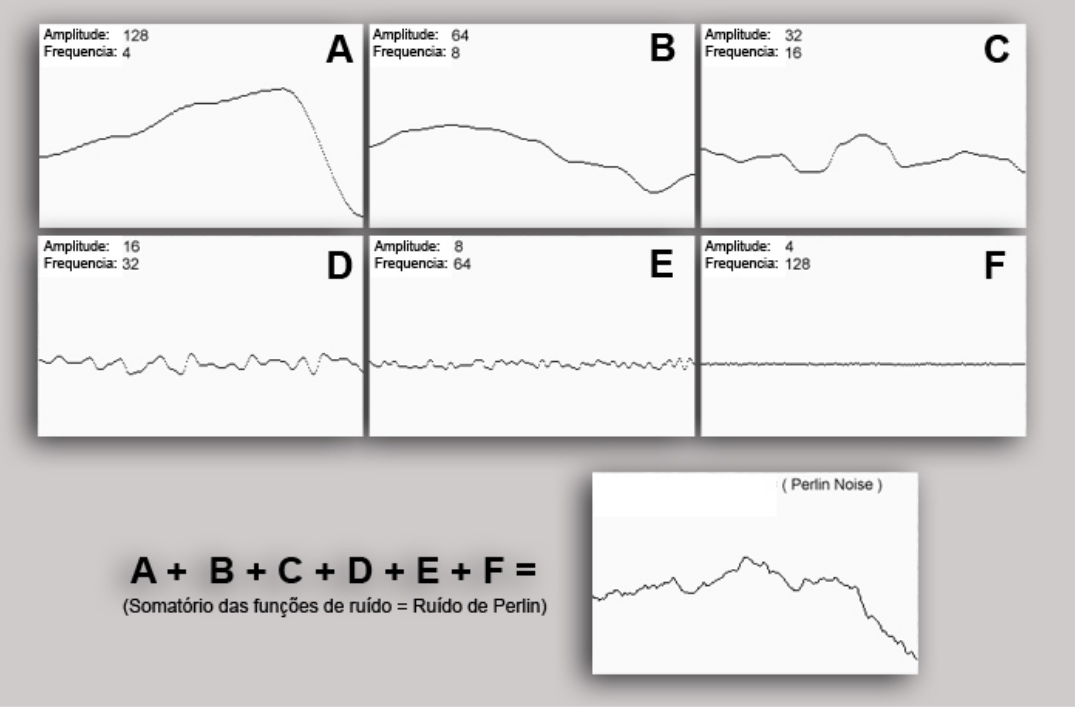
\includegraphics[width=.7\textwidth]{img/perlin1d.png}
%         \caption{Ruído de Perlin em uma dimensão.}
%   \end{figure}
% \end{frame}

\begin{frame}{Perlin Noise octaves}
    \begin{equation*}
        \begin{split} 
            \visible<+->{max & = \lim_{n\to \infty} 2^{-n} (2^{n +1}-1) \\}
            \visible<+->{& = 2}
        \end{split}
    \end{equation*}
\end{frame}

%mostrar dimenções e manipulações do ruido

%limitações, é realmente infinito?
